\documentclass[12pt, twoside]{article}
\documentclass[12pt, twoside]{article}
\usepackage[letterpaper, margin=1in, headsep=0.2in]{geometry}
\setlength{\headheight}{0.6in}
%\usepackage[english]{babel}
\usepackage[utf8]{inputenc}
\usepackage{microtype}
\usepackage{amsmath}
\usepackage{amssymb}
%\usepackage{amsfonts}
\usepackage{siunitx} %units in math. eg 20\milli\meter
\usepackage{yhmath} % for arcs, overparenth command
\usepackage{tikz} %graphics
\usetikzlibrary{quotes, angles}
\usepackage{graphicx} %consider setting \graphicspath{{images/}}
\usepackage{parskip} %no paragraph indent
\usepackage{enumitem}
\usepackage{multicol}
\usepackage{venndiagram}

\usepackage{fancyhdr}
\pagestyle{fancy}
\fancyhf{}
\renewcommand{\headrulewidth}{0pt} % disable the underline of the header
\raggedbottom
\hfuzz=2mm %suppresses overfull box warnings

\usepackage{hyperref}

\fancyhead[LE]{\thepage}
\fancyhead[RO]{\thepage \\ Name: \hspace{4cm} \,\\}
\fancyhead[LO]{BECA / Dr. Huson / Geometry\\*  Unit 10: Trigonometry \\* 5 May 2023}

\begin{document}

\subsubsection*{10.10 Special right triangles \hfill HSG.SRT.C.8}
\begin{enumerate}
\item Isosceles right $\triangle ABC$ is shown with legs $AC=BC=10$ as marked.\vspace{0.25cm}
  \begin{multicols}{2}
    \begin{enumerate}[itemsep=0.2cm]
      \item Write down $\theta$.
      \item Find the length of hypotenuse $AB$.\vspace{1cm}
      \item Write down $\tan A =$
      \item Find $\cos A =$
      \item Find $\sin A =$
    \end{enumerate}
    \begin{flushright}
      \begin{tikzpicture}[scale=0.9]
        \draw [thick](0,0)node[below]{$A$}--
        (5,0)node[below]{$C$}--
        (5,5)node[above right]{$B$}--cycle;
        \draw (5,0)++(-0.6,0)--++(0,0.6)--+(0.6,0);
        \node at (2.5,0)[below]{$10$};
        \node at (5,2.5)[right]{$10$};
        \draw [thick, -] (1,0) arc [start angle=0, end angle=45, radius=1];
        \node at (1.2,0.1)[above]{$\theta$};
      \end{tikzpicture}
    \end{flushright}
  \end{multicols} \vspace{1cm}

\item Given right triangle $\triangle ABC$ with base $AC=1$ and hypotenuse $AB=2$ as marked.\vspace{0.25cm}
\begin{enumerate}[itemsep=1.cm]
  \begin{multicols}{2}
    \item Find the altitude $BC=h$. \vspace{1cm}
    \item $\triangle ABC$ is reflected across $\overline{BC}$. Mark the lengths of the sides of its image $\triangle DBC$ 
    \item Write down the angle measure of $\angle A$.
\begin{flushright}
        \begin{tikzpicture}[scale=1]
        \draw [thick]
        (0,0)node[below]{$A$}--
        (3,0)node[below]{$C$}--
        (60:6)node[above]{$B$}--cycle;
        \draw (3,0)++(-0.5,0)--++(0,0.5)--+(0.5,0);
        \draw [dashed] (3,0)--(6,0)node[below]{$D$}--(60:6);
        \node at (1.5,0)[below]{$1$};
        \node at (62:3)[left]{$2$};
        \node at (3,2)[right]{$h$};
      \end{tikzpicture}
\end{flushright}
\end{multicols}
\item Write down the angle measure of $\angle ABC$.
\item Write down $\cos A$.
\item Write down $\sin A$.
\vspace{1cm}
\end{enumerate}
\vspace{1cm}

\newpage
\item Shown is a building with student $A$ on the ground waving up to student $B$. Point $A$ is 40 feet from the base of the building, and the angle of elevation from $A$ to $B$ is $37^\circ$.

Find how high up student B is from the ground to the \emph{nearest foot}. \hfill (not to scale)
  \begin{flushright}
    \begin{tikzpicture}[scale=0.3]
      %\draw [-, thick] (0,0)--(35:23);
      \draw [-, thick] (-4,0)--
      (0,0)--
        (17,0)--
        (22,0)--
        (22,10)--(17,10)--(17,0);
      \draw [fill] (0,0) circle [radius=0.1] node[above left]{$A$};
      \draw [fill] (17,10) circle [radius=0.1] node[above right]{$B$};
      \draw [dashed] (0,0)--(17,10);
      \node at (3.8, 0)[above]{$37^\circ$};
      \node at (11, 0)[above]{distance = 40 ft};
      \node at (19.5, 5)[above]{school};
    \end{tikzpicture}
    \end{flushright}

\item Yolanda is making a springboard to use for gymnastics. She has 8-inch-tall springs and wants to form a $16.5$ angle with the base, as modeled in the diagram below.
\begin{center}
  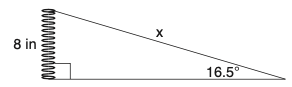
\includegraphics[scale=0.6]{../graphics/trig-spring.png}
\end{center}
To the \emph{nearest tenth of an inch}, what will be the length of the springboard, $x$? \vspace{4cm}

\item A child sleds from the top of a hill to a group of friends standing at the base of the hill. The hill is 20 feet tall, and the distance from the sledder to the group of friends is 110 feet. Find the angle of the incline $x$, to the \emph{nearest whole degree}.
\begin{flushright}
  \begin{tikzpicture}[scale=1.1]
    \draw [thick] (10,0)--(0,0)--(10,2.0)--cycle;
    \draw [thick, ->] (1.5,0) arc [start angle=0, end angle=11.3, radius=1.5];
    \node at (1,0)[below]{Incline $=x^\circ$};
    \node at (10,1.2)[left]{$20$};
    \node at (5,1.6)[below]{$110$};
  \end{tikzpicture} 
\end{flushright}\vspace{4cm}
  
\newpage
\item In the diagram below, $\triangle ABC$ is inscribed in circle $O$. Show that $\overline{AB} \perp \overline{BC}$.
    \begin{flushright}
      \begin{tikzpicture}[scale=0.6]
        \draw [help lines] (0,0) grid (10,7);
        \draw [thick, <->] (-0.4,0) -- (10.4,0) node [below right] {$x$};
        \draw [thick, ->] (0,0)--(0,7.4) node [left] {$y$};
        \draw [thick]
          (0,0)node[below]{$A$}--
          (2,4) node[above left]{$B$}--
          (10,0) node[below]{$C$}--cycle;
        \draw [fill] (5,0) circle [radius=0.1] node[below] {$O$};
        \clip (0,0) rectangle (10,6);
        \draw (5,0) circle [radius=5];
      \end{tikzpicture}
    \end{flushright} \vspace{1cm}

\item In the diagram below, $\triangle ABC$ has vertices with coordinates $A(1,2)$, $B(8,3)$ and $C(4, 6)$.
    \begin{center} %4 quadrant regents grid
      \begin{tikzpicture}[scale=.48]
        \draw [help lines] (-4,0) grid (9,7);
        \draw [thick, <->] (-4.4,0) -- (9.4,0) node [below right] {$x$};
        \draw [thick, <->] (0,-0.7)--(0,7.4) node [left] {$y$};
        \draw [thick]
          (1,2)node[below]{$A$}--
          (8,3) node[right]{$B$}--
          (4,6) node[above right]{$C$}--cycle;
        %\draw [fill] (-1,2) circle [radius=0.1] node[above left] {$A$};
        %draw [fill] (8, -4) circle [radius=0.1] node[below right] {$C$};
      \end{tikzpicture}
    \end{center}
    Find the length of each side of $\triangle ABC$, showing that it is isosceles and not equilateral.\\[0.5cm]
      \begin{tabular}{c|c|c}
        $AC=$ & $BC=$ & $AB=$ \\
        $\sqrt{(x_C-x_A)^2+(y_C-y_A)^2}$ & $\sqrt{(x_C-x_B)^2+(y_C-y_B)^2}$ & $ \sqrt{(x_B-x_A)^2+(y_B-y_A)^2}$ \\
        & & \\
        & & \\
      \end{tabular}

\newpage
\item The vertices of quadrilateral $MATH$ have coordinates $M(-4,2)$, $A(-1,-3)$, $T(9,3)$, and $H(6,8)$. \\[0.5cm]
Prove that quadrilateral $MATH$ is a parallelogram.


\end{enumerate}
\end{document}
  